\documentclass[journal,twoside,web]{ieeecolor}
\usepackage{jsen,wrapfig}
\usepackage[T1]{fontenc}
\usepackage{amsmath,amssymb,graphicx,booktabs,array,cite}
\usepackage[hidelinks]{hyperref}
\usepackage{url,xurl,balance}
% Allocate the running head its actual height without moving the text block.
\addtolength{\topmargin}{-5pt}\addtolength{\headheight}{5pt}
\definecolor{abstractbg}{rgb}{0.89804,0.94510,0.83137}
\setlength{\fboxrule}{0pt}\setlength{\fboxsep}{0pt}
\hypersetup{pdftitle={Accuracy, Storage, and Update Cost in Reference-Assisted Sensor Calibration},pdfauthor={Oleksandr Kuznetsov}}
\makeatletter\let\tableinput\@@input\makeatother
\interdisplaylinepenalty=2500
\setcounter{dbltopnumber}{3}
\renewcommand{\dbltopfraction}{0.88}
\renewcommand{\textfraction}{0.1}
\newcommand{\degC}{\ensuremath{^{\circ}\mathrm{C}}}
\newcommand{\us}{\ensuremath{\mu\mathrm{s}}}
\hyphenation{micro-controller micro-controllers mono-tonic}
\begin{document}
\title{Accuracy, Storage, and Update Cost in Reference-Assisted Sensor Calibration}
\author{\mbox{Oleksandr Kuznetsov,~\IEEEmembership{Member,~IEEE}}%
\thanks{O. Kuznetsov is with the Department of Theoretical and Applied Sciences, eCampus University, Italy, and with the Department of Intelligent Software Systems and Technologies, School of Computer Science and Artificial Intelligence, V.N. Karazin Kharkiv National University, Ukraine (e-mail: oleksandr.kuznetsov@uniecampus.it; ORCID: 0000-0003-2331-6326).}\endgraf}
\markboth{IEEE Sensors Journal}{Kuznetsov: Reference-Assisted Sensor Calibration}
\IEEEtitleabstractindextext{%
\fcolorbox{abstractbg}{abstractbg}{%
\begin{minipage}{\textwidth}%
\begin{wrapfigure}[12]{r}{3in}%
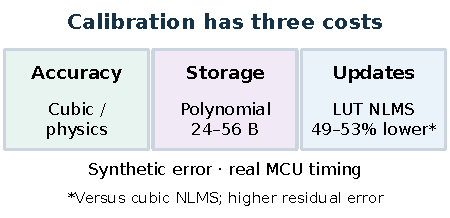
\includegraphics[width=3in]{figures/gagraphic_inline.pdf}%
\end{wrapfigure}%
\begin{abstract}
Embedded calibration requires separate decisions about approximation accuracy, stored model size, and the cost of incorporating new references. This paper compares lookup tables, compact cubic splines, expanded cubic polynomials, and fitted physical and global polynomial models. Synthetic thermistor and light-dependent-resistor cases provide controlled tests at 80, 144, and 224 bytes. Compact cubics are more accurate than float32 tables in 15 of 18 matched cells in the original study; physical models are strongest when their assumptions describe the complete response. Additional experiments evaluate cross-validation, generator sensitivity, decaying adaptation rates, blockwise least-squares affine correction, and causal batch refitting. They expose both selection instability and the conflict between tracking speed and stationary error. Physical Mega2560 and ESP32-C3 measurements include polynomial and physical references on a separate, fully identified fixture. A 56-byte polynomial is more accurate but slower than a 144-byte table on that fixture. On the matched fixture, ordinary normalized least-mean-square table updates take 48.7--53.3\% less time than compact cubic updates, with higher residual error. The evidence supports conditional resource trade-offs rather than an accuracy advantage for tables. Accuracy and drift are simulated; physical sensor uncertainty, energy, and worst-case execution time are not established.
\end{abstract}
\begin{IEEEkeywords}
Calibration, embedded systems, lookup tables, microcontrollers, sensor drift, splines.
\end{IEEEkeywords}
\end{minipage}}}
\maketitle
% Working submission copy: use the class's normal running head, with no
% publisher logo, fabricated volume/date, or publication copyright line.
\thispagestyle{headings}

\section{Introduction}
\IEEEPARstart{S}{ensor} calibration maps an electrical observation to a physical quantity. The mapping may be evaluated thousands of times between reference measurements, or updated during scheduled maintenance. These two operations have different costs. A small equation may require logarithms at every inference; a larger table may evaluate quickly; an adaptive model may need more state than its inference payload suggests. Selecting a representation therefore requires accuracy, storage, and execution costs to be considered together.

Software sensor linearization is established. Erdem compared accuracy, memory, and time on low-cost microcontrollers \cite{erdem}; Petkov\v{s}ek \emph{et al.} studied thermistor equations, tables, and polynomial evaluation for time-critical measurements \cite{petkovsek}. Piecewise-linear sensor approximation also addresses segment placement and prescribed error limits \cite{marinov}. The 2004 IEEE 1451.4 standard specifies transducer electronic data sheets (TEDS) \cite{teds}; its calibration-table and calibration-curve templates represent tabulated pairs and polynomial segments \cite{ni}. This motivates explicit storage accounting, although the payloads here are internal representations, not compliant TEDS records.

Reference availability is a separate question. In situ sensor calibration includes architectures that obtain information from reference instruments or neighboring sensors \cite{delaine}. Long-term chemical-sensor drift has been evaluated using physical recordings collected over years \cite{vergara}. Such experiments address phenomena that a prescribed numerical disturbance cannot validate. Adaptive spline filtering, normalized least mean squares (NLMS), recursive least squares (RLS), and isotonic projection provide established algorithms \cite{scarpiniti,haykin,pava}. On-device neural training further demonstrates that update memory must be counted separately from inference memory \cite{tinytrain}.

The contribution here is an implementation and evaluation study, not a new approximation or adaptation algorithm. It combines byte-exact inference accounting, common reference streams, stored-precision validation, and physical microcontroller timings. Additional analyses test sensitivity to generator assumptions and model selection, and compare sequential updates with simpler correction and larger-memory refits. The resulting recommendation is conditional: fitted physical models and compact cubics often have better accuracy, while tables can reduce computation. Figure~\ref{fig:protocol} distinguishes numerical calibration evidence from physical execution measurements. No acquired sensor readings enter the accuracy study.

\begin{figure*}[!t]
\centering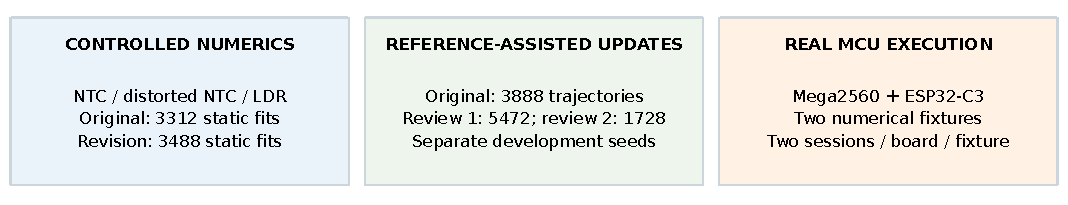
\includegraphics[width=\textwidth]{figures/protocol.pdf}
\caption{Evidence inventory. Numerical cases determine accuracy; physical boards determine execution time. Revision analyses use separate development and confirmation seeds; the affine/decay refinement reuses them. Both hardware fixtures have independent identities and are kept separate.}
\label{fig:protocol}
\end{figure*}

\section{Representations and Fitting}
\subsection{Payload and function class}
\normalcolor
Let $a$ denote the normalized analog-to-digital converter (ADC) observation and $q$ the reference quantity. The transforms $x=(a-a_m)/a_h$ and $y=(q-q_m)/q_h$ store four float32 values, consuming 16 bytes. The input half-range is expanded by 5\% using only initial observations. The output transform uses the specified operating range. Transforms remain fixed during recalibration.

For fixed basis functions, $\hat y=\boldsymbol b(x)^T\boldsymbol c$. A uniform lookup table (LUT) uses two linear hat functions; a compact cubic B-spline uses four local basis functions \cite{deboor}. Expanded cubic pieces use local $u\in[0,1]$ and
\begin{equation}
 p_j(u)=((c_{j,3}u+c_{j,2})u+c_{j,1})u+c_{j,0}.
 \label{eq:horner}
\end{equation}
The expanded model is converted from a $C^2$ source spline. Its stored piece coefficients are redundant: $P$ pieces originate from $P+3$ source coefficients, not $4P$ independently fitted parameters. Thus ``4/7'' in Table~\ref{tab:payload} means four pieces from seven source coefficients. This is a restricted smooth representation, not a general free piecewise-cubic competitor. Comparisons against compact cubics avoid attributing an accuracy advantage to that storage redundancy.

\begin{table}[t]
\caption{Exact Inference Payload Configurations}
\label{tab:payload}\centering\footnotesize
\begin{tabular}{lrrr}\toprule
Representation & 80 B & 144 B & 224 B\\\midrule
Float32 LUT: nodes &16&32&52\\
Affine int16 LUT: nodes &28&60&100\\
Compact cubic: coefficients &16&32&52\\
Expanded Horner: pieces/source coefficients &4/7&8/11&13/16\\\bottomrule
\end{tabular}
\end{table}

Float32 tables and compact splines occupy $16+4N$ bytes. The int16 table uses $24+2N$, including scale and offset. Expanded pieces use $16+16P$. Uniform knots and dimensions are implicit compile-time constants. These counts exclude code, stack, fitting workspace, and the test fixture. Selected global Chebyshev polynomials occupy 24--56 bytes; fitted Steinhart--Hart and log-linear resistance models occupy 32 and 28 bytes, respectively \cite{steinhart}. They receive the same references and no hidden generator parameters.

\subsection{Objective, selection, and convexity}
\normalcolor
The initial fit minimizes a penalized least-squares objective \cite{eilers}:
\begin{equation}
 \mathcal L(\boldsymbol c)=\frac{\|A\boldsymbol c-\boldsymbol y\|_2^2}{B_{\rm fit}}
 +\frac{\lambda\|D_2\boldsymbol c\|_2^2}{N-2},
 \label{eq:fit}
\end{equation}
where $B_{\rm fit}$ is the number of references used in that particular fit, $A$ is the fixed design matrix, and $D_2$ is the second-difference matrix. With $\lambda\geq0$, the Hessian is positive semidefinite. For $\lambda>0$, strict convexity requires $\ker A\cap\ker D_2=\{0\}$; at $\lambda=0$, full column rank of $A$ is required. Decreasing coefficient constraints form a convex set. Integer encoding and the discrete choice of hyperparameters are separate operations; they are not covered by this convexity statement.

The smoothing grid is $\{0,10^{-6},10^{-4},10^{-2},1,100\}$. Polynomial degrees are $\{1,2,3,4,5,7,9\}$. The original selector holds out every third interior reference. All labels, including validation labels, count toward the budget $B$; the selected model is refitted on all $B$ references. Selection evaluates the declared storage encoding. Additional float32 analyses compare this selector with fivefold interleaved cross-validation using the same candidates and total $B$, again followed by a full-data refit. Test labels are never used for selection. Fitting and update pseudocode are in the supplement.

\section{Controlled Numerical Protocol}
\subsection{Sensor responses and error measures}
\normalcolor
The negative-temperature-coefficient thermistor (NTC) response over $0$--$100\,\degC$ is
\begin{equation}
\begin{aligned}
 R(q)&=R_0\exp\!\left[\beta\left(\frac1{q+273.15}-\frac1{298.15}\right)\right],\\
 a&=R(q)/(10\,000+R(q)).
\end{aligned}
\label{eq:ntc}
\end{equation}
Virtual units draw $R_0=10\,\mathrm{k}\Omega\pm5\%$ and $\beta=3950\,\mathrm{K}\pm3\%$ uniformly. A paired front-end case adds $(4/1023)\sin(6\pi a+\phi)$, with uniform $\phi\in[-\pi,\pi]$. The light-dependent resistor (LDR) uses $q=\log_{10}(\mathrm{lux})\in[0,3]$, $R=R_0(10/10^q)^\gamma$, $R_0=10\,\mathrm{k}\Omega\pm30\%$, and $\gamma=0.7\pm10\%$. These are declared generator assumptions, not measured manufacturing distributions.

Each ADC observation averages 16 independently noisy, rounded, clipped 10-bit conversions. Per-conversion Gaussian noise has standard deviation one least significant bit (LSB). Initial reference noise is $0.02\,\degC$ or $0.005\log_{10}(\mathrm{lux})$. Budgets $B=30,75$ cover the operating range with bounded interior jitter. Independent evaluation uses the 401 interior points of a 403-point quantity grid.

We report ideal-input mean absolute error (MAE), noisy-input MAE, and the largest error observed on the finite test grids. Ideal-input error still includes fitting and reference-noise effects; it is not pure interpolation error. A further benchmark inverts the exact generator on noisy ADC observations, clipped to the operating range. This oracle inverse measures the error propagated by the assumed observation process. It is neither a universal statistical lower bound nor a measurement-uncertainty estimate. MAE components cannot be subtracted as additive uncertainty terms.

The original experiment has eight virtual units and three repetitions per scenario and budget: 144 cases and 3312 static evaluations. Its additional comparators include monotone LUTs and a scalar spline-plus-SiLU edge; complete results remain in the supplement. The latter is retained only for continuity with earlier LUT compilation work \cite{kan,lutkan}, not as a central sensor-calibration claim. Repetitions are averaged within each unit. Original unit-bootstrap intervals describe the simulator; they provide no estimate of manufactured-sensor population uncertainty.

The revision uses a new seed, eight units, and two repetitions. Nominal fits compare both selection procedures. One-factor-at-a-time analyses vary ADC noise to 0.25 or 4 LSB, tolerance half-widths to 0.5 or twice nominal, front-end distortion to 1 or 12 LSB, and its frequency to one or nine cycles over normalized ADC. The last two factors apply only to distorted NTC. Seeds are paired across settings. There are 608 cases and 3488 fitted-model evaluations, with all settings retained; interactions between factors are not tested.

\subsection{Reference-assisted sequential recalibration}
\normalcolor
Each stream supplies 384 labelled references spanning the range in shuffled 32-bin blocks. This models access to a controlled reference source during recalibration. It does not demonstrate autonomous drift detection or compensation without labels. Drift is absent, a step at sample 128, or a ramp from samples 128 to 256:
\begin{equation}
 \Delta a_t=\frac{d_t}{1023}[2+2\sin(2\pi a)],\qquad 0\leq d_t\leq1.
 \label{eq:drift}
\end{equation}
At $d_t=1$, the disturbance ranges from 0 to 4 LSB. Although smooth, it varies with ADC input, so it is not a constant offset. It is not an aging law.

LUT32 and cubic32 use identical fixed transforms and their own initial 144-byte fits. NLMS updates are
\begin{equation}
 \boldsymbol c_{t+1}=\boldsymbol c_t+
 \eta_t\frac{(y_t-\boldsymbol b_t^T\boldsymbol c_t)\boldsymbol b_t}
 {\boldsymbol b_t^T\boldsymbol b_t+10^{-6}}.
 \label{eq:nlms}
\end{equation}
The usual normalized-step interval is $0<\eta_t<2$ under standard stationary assumptions \cite{haykin}. Identification of all coefficients also requires sufficient excitation. Noisy inputs, noisy labels, finite precision, and changing targets preclude an unconditional convergence claim; constant steps can leave steady-state misadjustment. Projected variants apply the pool-adjacent-violators algorithm (PAVA) to decreasing coefficients. This is sufficient, but not necessary, for a monotone cubic spline.

The original nine methods are frozen LUT/cubic/polynomial, plain and projected LUT/cubic NLMS, and full-covariance cubic/polynomial RLS. Separate development selects $\eta=0.5$ and forgetting factor 0.98. RLS initializes $P_0=100I$, symmetrizes its covariance, and stores state as float32. Confirmation contains 432 streams and 3888 trajectories.

The revision retains these methods and adds decaying NLMS, blockwise least-squares affine correction, and batch refits. Rates $\eta_t=0.5/(1+t/\tau)$ select $\tau\in\{32,128,512,1024,2048\}$ on development data. Every completed 32-label block fits $y\simeq gp+o$ by ordinary least squares using all frozen predictions $p$ and their reference labels. It accumulates $\sum p$, $\sum y$, $\sum p^2$, and $\sum py$ in float32, stores gain/offset in float32, then resets the sums. The correction is held until the next block completes; no future labels enter it. A float64-accumulation audit checks numerical sensitivity. Batch models refit on either all initial-plus-prefix references or the latest 64, at the 15 fixed evaluation checkpoints, retaining the initial smoothing parameter. These are larger-memory accuracy baselines, not equal-state MCU implementations. RLS selection is extended to $\{0.90,0.95,0.98,0.995,1\}$.

The development criterion is checkpoint-integrated normalized mean squared error over all scenarios, budgets, and schedules, including no drift. The first revision evaluated 2304 development and 5472 confirmation trajectories, selecting cubic RLS 0.98 and polynomial RLS 0.95. The subsequent affine-estimator and decay-grid changes reuse those seeds for a paired post-review reanalysis: 1440 development trajectories select $\tau=2048$ for both families, and 1728 confirmation trajectories evaluate decay and both accumulation precisions. Development and confirmation streams remain separate, but these are not a new untouched confirmation sample. The decay parameter is again at the boundary. Over 384 references, $\eta_t$ falls only from 0.5 to 0.421 (15.8\%); the criterion therefore favors a nearly constant step over this horizon, not an identified decay timescale. The grid is now fixed, with no further selection on these confirmation seeds. All runs and the earlier $\tau=512$ results are retained. No numerical failures occurred. The protocols were frozen locally before each computation, not publicly preregistered.

\section{Numerical Results}
\subsection{Accuracy and capacity}
\normalcolor
In the original study, compact cubic splines are more accurate than float32 LUTs in 15 of 18 matched scenario--budget--payload cells. The three exceptions have 224-byte models and $B=30$; expanded Horner is more accurate than either in those cells. No LUT variant has the lowest MAE in any of the 18 cells. At 80 bytes, compact cubics have 37.9--52.9\% lower noisy MAE than float32 LUTs. The observed LUT-versus-expanded-Horner crossing at low storage concerns the restricted $C^2$ expansion only; it does not establish LUT accuracy superiority. Selected 24--56-byte polynomials match or beat the best LUT across all tested sizes and variants in five of six scenario--budget groups. A well-specified physical model should be tested first.

Table~\ref{tab:errors} separates error components for the new nominal confirmation cases. At $B=75$, the oracle noisy-inverse MAE is $0.0404\,\degC$ for NTC, $0.0403\,\degC$ for distorted NTC, and $0.00106\log_{10}(\mathrm{lux})$ for LDR. Thus, observation noise compresses differences visible under ideal inputs. The finite-grid maxima are much larger than the means and are not certified worst-case bounds.

\begin{table*}[!t]
\caption{Revision Nominal Cases, $B=75$: Ideal and Noisy MAE, and Maximum Observed Noisy Error}
\label{tab:errors}\centering\small
\begin{tabular}{llrrr}\toprule
Scenario & Model & Ideal MAE & Noisy MAE & Maximum observed\\\midrule
\tableinput tables/revision_static.tex
\bottomrule\end{tabular}\par\vspace{3pt}
\footnotesize NTC errors are in \degC; LDR errors are in $\log_{10}(\mathrm{lux})$. LUT/cubic: 144 B and fivefold selection; polynomial: selected smaller payload; physics: fitted parameters. Means average eight units with two repetitions; maxima span all 16 cases and test points.
\end{table*}

\begin{figure*}[!t]
\centering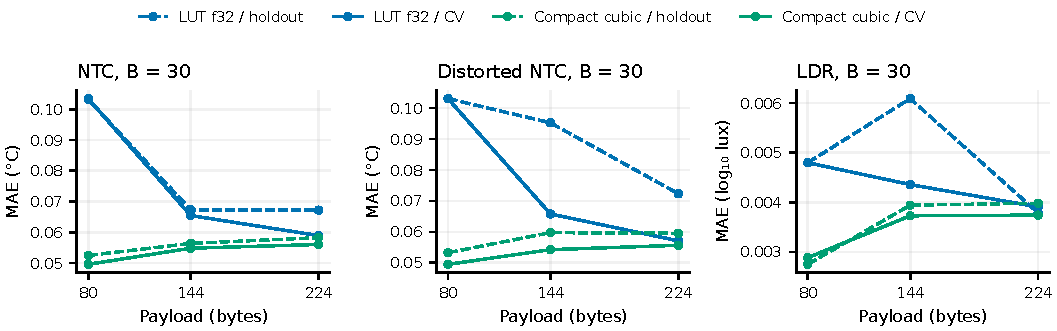
\includegraphics[width=\textwidth]{figures/cv_capacity.pdf}
\caption{Effect of selection at 30 initial references, new confirmation seed. Cross-validation reduces several high-capacity failures but does not make increasing model size uniformly beneficial. Physical units differ across panels.}
\label{fig:cv}
\end{figure*}

Cross-validation reduces some selection failures (Fig.~\ref{fig:cv}). For distorted NTC with $B=30$, the 144-byte LUT improves from $0.0952$ to $0.0658\,\degC$ noisy MAE; its largest observed error falls from 11.6 to $0.702\,\degC$. However, cross-validation is not universally better: the polynomial in that group worsens from $0.0541$ to $0.0732\,\degC$. Even with cross-validation, cubic NTC MAE at $B=30$ rises from $0.0496\,\degC$ at 80 bytes to $0.0560\,\degC$ at 224 bytes. Finite noisy references and the fixed smoothing grid still limit effective capacity.

\begin{figure*}[!t]
\centering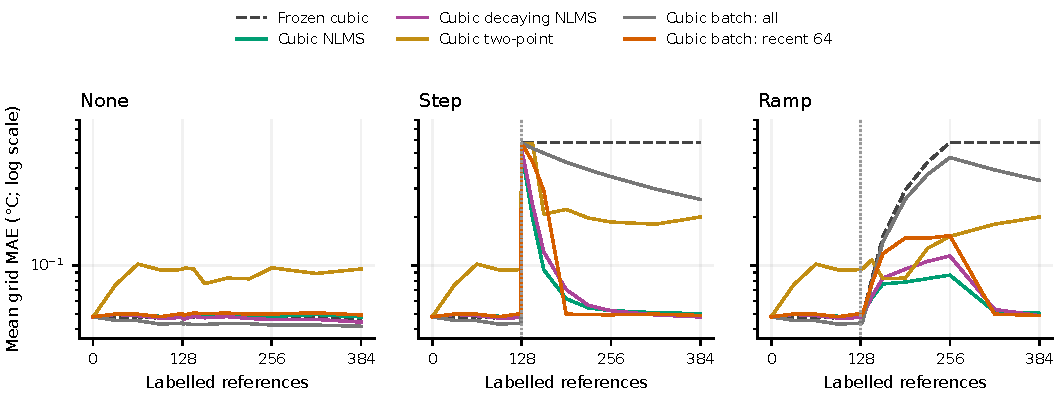
\includegraphics[width=\textwidth]{figures/revision_adaptation.pdf}
\caption{Paired reanalysis: distorted NTC, 75 initial labels. Decaying NLMS uses $\tau=2048$; block OLS uses all 32 pairs. Curves join post-update errors at fixed checkpoints; they do not resolve intermediate transients. All-history refits average incompatible pre/post-drift data. Recent-window refits need a reference buffer and are not timed on the boards.}
\label{fig:adapt}
\end{figure*}

\subsection{Tracking versus stationary error}
\normalcolor
Figure~\ref{fig:adapt} compares the new causal baselines on distorted NTC with $B=75$. Without drift, cubic batch refitting on all references reaches $0.0417\,\degC$, versus $0.0468\,\degC$ frozen and $0.0477\,\degC$ with constant-step NLMS. With the expanded-grid choice, decaying NLMS reaches $0.0465\,\degC$; block OLS reaches $0.0484\,\degC$. Thus, extra labels are useful, but constant-step updating need not extract their full stationary benefit.

After step drift, decaying cubic NLMS reaches $0.0489\,\degC$, versus $0.0500\,\degC$ with the fixed rate. Its integrated MAE is slightly worse, 0.0706 versus $0.0699\,\degC$. All-history batch refitting retains stale pre-drift references and ends at $0.257\,\degC$; the recent-64 refit reaches $0.0487\,\degC$. Block OLS reaches $0.0730\,\degC$ after both step and ramp drift, markedly improving on the previous two-endpoint correction ($0.199\,\degC$). Its integrated MAE is $0.0966\,\degC$ for the step and $0.0692\,\degC$ for the ramp. In the ramp case it also improves on cubic RLS ($0.101\,\degC$). Thus sequential local updates retain a lower final error, but their advantage over a well-estimated affine correction is substantially smaller.



Extending the forgetting-factor grid reduces the polynomial RLS integrated step error from 0.104 to $0.0756\,\degC$ in this group, but worsens its final error from 0.0467 to $0.0501\,\degC$. Cubic RLS remains at 0.98. Selection optimized a global integrated criterion, not each individual endpoint. Full tables retain both settings and all schedules.

\subsection{Sensitivity and constraint activity}
\normalcolor
\begin{figure}[t]
\centering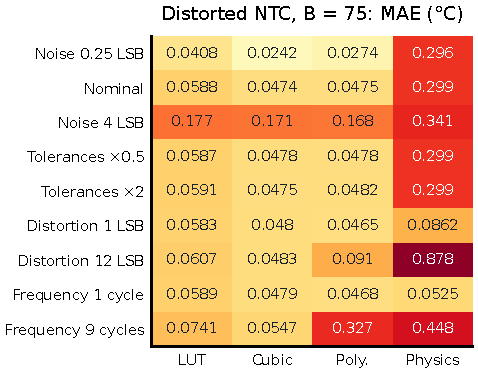
\includegraphics[width=\columnwidth]{figures/sensitivity.pdf}
\caption{Sensitivity to one generator factor at a time. Nominal values are noise 1 LSB, original tolerance ranges, distortion 4 LSB, and three cycles. Colors encode MAE on a logarithmic scale; cell values are in \degC. LUT/cubic use 144 B.}
\label{fig:sensitivity}
\end{figure}

Sensitivity changes which small model is adequate (Fig.~\ref{fig:sensitivity}). At nine disturbance cycles, polynomial MAE increases to $0.327\,\degC$, versus $0.0547\,\degC$ for cubic and $0.0741\,\degC$ for LUT. At 12 LSB amplitude, the corresponding values are 0.0910, 0.0483, and $0.0607\,\degC$. These stress cases show where local flexibility helps; they do not establish that actual front ends exhibit these disturbances. At 4 LSB noise, observation error dominates and the three numerical models approach one another.

Replaying every projected update in the original experiment gives no changed LUT state in 165888 updates. Cubic projection changes 42 initial states and 557 updates across 42 of 432 trajectories. Projected LUT is therefore redundant in this regime; projection is not presented as an accuracy contribution. Coefficient monotonicity should be checked cheaply before invoking PAVA when the constraint is required. The supplied guarded implementation is tested, but its hardware time is not measured.

\begin{figure*}[!t]
\centering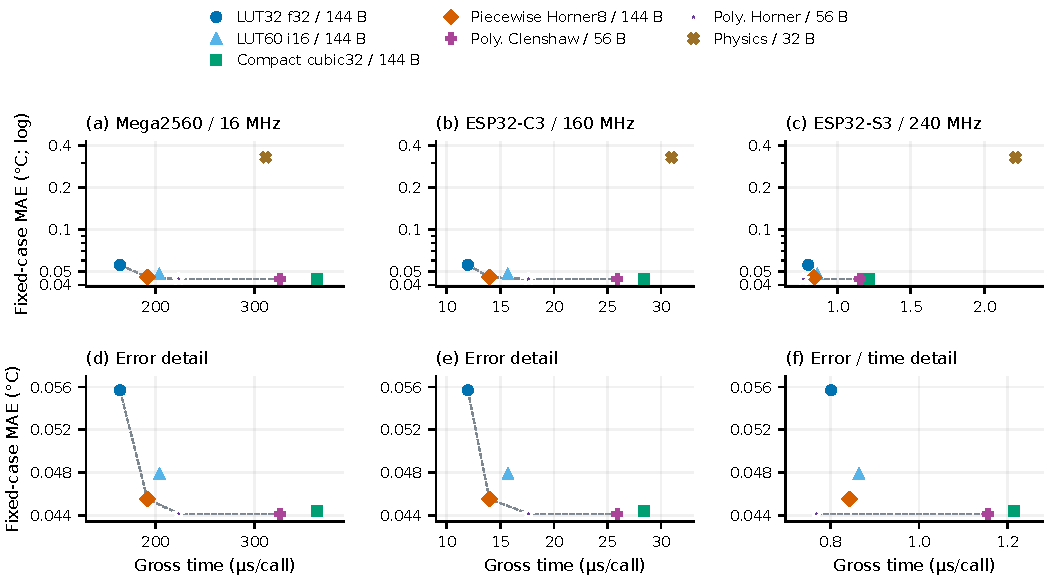
\includegraphics[width=\textwidth]{figures/hardware_complete.pdf}
\caption{Physical MCU time and synthetic error. Top: the earlier pilot includes physical and polynomial references at their actual payloads (logarithmic error axis). Bottom: the separate matched 144-byte fixture. Points cannot be combined across rows into one frontier. Generic recursive cubic and scalar KAN pilot timings remain in the public archive; the compact spline shown uses specialized local evaluation.}
\label{fig:hardware}
\end{figure*}

\section{Physical Microcontroller Execution}
\subsection{Two identified fixtures}
\normalcolor
One Mega2560 at 16 MHz and one ESP32-C3 at 160 MHz execute synthetic inputs. Each fixture has two warm, command-driven sessions per board after one upload, with ten batches of 2048 calls per static method. Times below are medians of the two session medians. They include fixture reads and checksum accumulation, and exclude ADC acquisition and serial output. Raw logs, parsed records, sidecar hashes, and record counts are checked before use.

The earlier pilot fixture (seed 20261108, distorted NTC, unit 0, repetition 0, $B=75$) includes fitted physics, a degree-9 Chebyshev polynomial evaluated by Clenshaw recurrence, tables, and a 16-coefficient spline in compact and expanded forms. These measurements were recovered from existing captures, not generated by host simulation. The later matched fixture (seed 2026110801, otherwise the same identifiers) compares four 144-byte models and complete NLMS updates. Its coefficients, input values, and errors differ. Figure~\ref{fig:hardware} keeps the two fixtures in separate rows. They cannot provide a single comparison across all models. A new common-fixture acquisition is required for that purpose; its supplied firmware includes all four matched models, fitted physics, and the same degree-9 polynomial evaluated by both Clenshaw and power-basis Horner. Each polynomial payload is 56 bytes. Host parity and three target builds pass, but these are not additional board measurements.



\subsection{Inference and update costs}
\normalcolor
In the pilot, LUT float32 takes 155~\us{} on Mega2560 and 11.0~\us{} on ESP32-C3, versus 325 and 25.8~\us{} for the 56-byte polynomial. LUT MAE is $0.0524\,\degC$, versus $0.0476\,\degC$ for the polynomial. The polynomial saves payload and improves accuracy, while the LUT reduces time. Fitted thermistor physics takes 314 and 31.1~\us{}, with $0.267\,\degC$ MAE because it omits front-end distortion. This fixture does not establish its performance on a correctly specified physical chain.

The matched LUT32 takes 167 versus 193~\us{} for Horner8 on Mega2560 and 12.1 versus 14.0~\us{} on ESP32-C3: 13.2--13.8\% less time. MAE rises from 0.0455 to $0.0557\,\degC$, and maximum error from 0.268 to $0.470\,\degC$. Compact cubic32 has MAE $0.0444\,\degC$ at 369 and 28.5~\us. Its kernel uses local indexing and six unrolled de Boor interpolations, not generic knot search. Pre-expanding all 29 pieces would require $16+29\times16=480$ bytes, rather than 144; caching them is a different memory budget. Optimality among all equivalent kernels is not claimed.

\begin{table}[t]
\caption{Matched Step Fixture: Gross Time per Labelled Update}
\label{tab:updates}\centering\footnotesize
\begin{tabular}{lrrr}\toprule
Method & Mega (\us{}) & C3 (\us{}) & Final MAE (\degC)\\\midrule
LUT NLMS &371&24.6&0.0589\\
Cubic NLMS &724&52.7&0.0446\\
LUT NLMS + PAVA &797&43.8&0.0589\\
Cubic NLMS + PAVA &1150&71.9&0.0446\\\bottomrule
\end{tabular}
\end{table}

Ordinary LUT NLMS takes 48.7\% and 53.3\% less time than ordinary cubic NLMS (Table~\ref{tab:updates}), with higher final error. Each timing batch executes the entire 384-label trajectory, including normalization, basis evaluation, prediction, and coefficient writes. Initialization and validation are outside timing. All fixture states already meet the coefficient order, so full PAVA adds overhead without changing the result. Its measured time is not a worst-case projection bound.

Block OLS needs 16 bytes for the four float32 sums plus 8 bytes for gain/offset, a block counter, and the frozen model; 16 bytes is not its total state. Both NLMS models use 148 bytes of persistent state; full PAVA adds 160 bytes of reusable workspace. Cubic RLS needs 4244 bytes, and polynomial RLS up to 460 bytes, including covariance. A 64-pair float32 reference window alone needs 512 bytes, before model and solver workspace; an all-history buffer at $B=75$ needs 3672 bytes after 384 labels. Such batch references are not equal-memory competitors. Code size, payload, scratch, and call stack remain separate. The supplement gives absolute deployment-build sizes.

\section{Engineering Scope and Limitations}
The inference saving can be small in a slow acquisition cycle. For an illustrative AVR configuration with prescaler 128 at 16 MHz and 13 ADC cycles per steady-state conversion \cite{adc}, 16 conversions take 1664~\us. Including the measured matched kernels gives 1831~\us{} with LUT and 1857~\us{} with Horner: about 1.37\% total reduction. This is an analytical budget, not a measured acquisition loop; it omits software acquisition overhead, first-conversion startup, settling, communication, and sensor dynamics. The gain matters more when conversion results are already buffered, many channels share a processor, or reference updates compete with other tasks. No industrial deadline or energy saving is established.

Both measured processors use software floating-point arithmetic; the ESP32-C3 implements RV32IMC \cite{c3}. Hardware single-precision floating point on targets such as ESP32-S3 can change the balance \cite{fpu}. An optional S3 acquisition environment is supplied, but there are no S3 results here. One board per architecture, two warm sessions, and median gross timing do not establish device-to-device variation, interrupt sensitivity, worst-case execution time, measured peak stack, or energy per call. Identical rounded session medians do not imply zero raw timing dispersion.

The dominant limitation is metrological. Self-heating, ADC integral/differential nonlinearity, reference-voltage drift, thermal lag, lead resistance, and actual batch variation are not identified by this generator. A physical campaign must compare several sensor units against a calibrated reference, retain heating/cooling and repeat-cycle effects, and propagate reference, acquisition, stability, and spatial-gradient uncertainties \cite{gum,aranda}. Regression MAE alone is not that uncertainty budget. The supplement outlines a physical validation campaign and the required uncertainty components.

The numerical findings also depend on full-range references, uniform knots, fixed selection grids, and finite observation schedules. The sensitivity analysis varies one factor at a time and cannot exclude interactions. Blockwise output-affine regression does not exhaust ADC-domain correction, forgetting-weighted regression, or other reference schedules. The hardware frontier includes selected implementations, not every polynomial degree or fixed-point design. The illustrative three-candidate decision map is therefore retained only in the supplement.

\section{Conclusion}
Byte-exact storage and complete update costs expose useful trade-offs, but do not establish LUT accuracy superiority. Compact cubics and suitable physical or polynomial models provide strong accuracy baselines. Existing physical-MCU measurements show that a smaller, more accurate polynomial can take longer than a table, while ordinary table NLMS updates are faster than cubic updates at higher residual error. Cross-validation reduces some fitting failures; decaying rates and recent-data refits improve stationary or final accuracy while changing transient behavior and memory use. These results guide implementation choices within the declared numerical and hardware settings. Physical sensor validation remains necessary before transferring the error claims to an instrument.

\section*{Data and Code Availability}
Protocols, source, summaries, per-unit values, plot inputs, raw MCU logs, and audits are public in the project repository \cite{code}. Original evidence is fixed at commit \texttt{db39238}, first-review analyses at \texttt{0b828da}, and the paired refinements at \texttt{45edb31}. The source package includes exact plot inputs and hashes. The complete 234 MB evidence package is openly available in Zenodo, version 1.0.0, doi: \href{https://doi.org/10.5281/zenodo.24062383}{10.5281/zenodo.24062383} \cite{data}. It preserves the original and both revision archives, the research code at \texttt{45edb31}, and SHA-256 manifests. The supplemental material distinguishes original results, new analyses, and prospective hardware work.

\section*{Acknowledgment}
OpenAI ChatGPT assisted with manuscript and supplementary drafting, experiment-design refinement, simulation and analysis code, embedded firmware and acquisition tooling, validation scripts, and visualization code. Numerical figures are generated from preserved records, not image-generation models.
\begin{thebibliography}{12}
\bibitem{erdem} H. Erdem, ``Implementation of software-based sensor linearization algorithms on low-cost microcontrollers,'' \emph{ISA Trans.}, vol. 49, no. 4, pp. 552--558, 2010, doi: \href{https://doi.org/10.1016/j.isatra.2010.04.004}{10.1016/j.isatra.2010.04.004}.
\bibitem{petkovsek} M. Petkov\v{s}ek, M. Nemec, and P. Zajec, ``Algorithm execution time and accuracy of NTC thermistor-based temperature measurements in time-critical applications,'' \emph{Mathematics}, vol. 9, no. 18, Art. no. 2266, 2021, doi: \href{https://doi.org/10.3390/math9182266}{10.3390/math9182266}.
\bibitem{steinhart} J. S. Steinhart and S. R. Hart, ``Calibration curves for thermistors,'' \emph{Deep Sea Res. Oceanogr. Abstr.}, vol. 15, no. 4, pp. 497--503, 1968, doi: \href{https://doi.org/10.1016/0011-7471(68)90057-0}{10.1016/0011-7471(68)90057-0}.
\bibitem{deboor} C. de Boor, ``On calculating with B-splines,'' \emph{J. Approx. Theory}, vol. 6, no. 1, pp. 50--62, 1972, doi: \href{https://doi.org/10.1016/0021-9045(72)90080-9}{10.1016/0021-9045(72)90080-9}.
\bibitem{eilers} P. H. C. Eilers and B. D. Marx, ``Flexible smoothing with B-splines and penalties,'' \emph{Statist. Sci.}, vol. 11, no. 2, pp. 89--121, 1996, doi: \href{https://doi.org/10.1214/ss/1038425655}{10.1214/ss/1038425655}.
\bibitem{scarpiniti} M. Scarpiniti, D. Comminiello, R. Parisi, and A. Uncini, ``Nonlinear spline adaptive filtering,'' \emph{Signal Process.}, vol. 93, no. 4, pp. 772--783, 2013, doi: \href{https://doi.org/10.1016/j.sigpro.2012.09.021}{10.1016/j.sigpro.2012.09.021}.
\bibitem{haykin} S. Haykin, \emph{Adaptive Filter Theory}, 5th ed. Upper Saddle River, NJ, USA: Pearson, 2014.
\bibitem{pava} J. de Leeuw, K. Hornik, and P. Mair, ``Isotone optimization in R: Pool-adjacent-violators algorithm (PAVA) and active set methods,'' \emph{J. Stat. Softw.}, vol. 32, no. 5, pp. 1--24, 2009, doi: \href{https://doi.org/10.18637/jss.v032.i05}{10.18637/jss.v032.i05}.
\bibitem{kan} Z. Liu \emph{et al.}, ``KAN: Kolmogorov--Arnold networks,'' in \emph{Proc. Int. Conf. Learn. Representations (ICLR)}, 2025. [Online]. Available: \url{https://arxiv.org/abs/2404.19756}
\bibitem{lutkan} O. Kuznetsov, ``LUT-KAN: Segment-wise LUT quantization for fast KAN inference,'' arXiv:2601.03332, 2026, doi: \href{https://doi.org/10.48550/arXiv.2601.03332}{10.48550/arXiv.2601.03332}.
\bibitem{gum} Joint Committee for Guides in Metrology, \emph{Evaluation of Measurement Data---Guide to the Expression of Uncertainty in Measurement}, JCGM 100:2008, 2008 (corrected 2010). [Online]. Available: \url{https://www.bipm.org/documents/20126/2071204/JCGM_100_2008_E.pdf}
\bibitem{code} O. Kuznetsov, ``LUT-native KAN: Sensor calibration comparison and MCU evidence,'' GitHub, commit \texttt{db39238}, Nov. 8, 2026. [Online]. Available: \href{https://github.com/KuznetsovKarazin/lut-kan-native/tree/db39238c1467169b65ff1f3581945e57ee7ffd7a/experiments/sensor_recovery}{github.com/KuznetsovKarazin/lut-kan-native}, experiment directory \texttt{experiments/sensor\_recovery}.
\end{thebibliography}

\end{document}
